%
% Manual for NodePoint - (C) 2015 Patrick Lambert
% Compile with XeLaTeX
%

% Document class
\documentclass[11pt]{article}
\usepackage{geometry}
\usepackage{listings} 

% Conditional compilation for Windows and Linux
\usepackage{ifthen}
\newboolean{Windows}
\setboolean{Windows}{true} % change to false for Linux
\ifthenelse{\boolean{Windows}}
{\def\NodePointManual{NodePoint IT System - Windows version 1.6.0}}
{\def\NodePointManual{NodePoint IT System - Linux version 1.6.0}}

% Margins and paper type
\geometry{a4paper, right=1.5cm, left=1.5cm, top=2cm, bottom=1.5cm}

% Color definitions
\usepackage{color}
\usepackage{hyperref}
\definecolor{headings}{rgb}{0,0.53,0.84}
\hypersetup{colorlinks, linkcolor={blue}, citecolor={blue}, urlcolor={blue}}

% Paragraph indent and spacing
\usepackage[english]{babel}
\setlength{\parindent}{0em}
\setlength{\parskip}{1em}
\usepackage{indentfirst}
\usepackage{setspace}

% Section titles
\usepackage{titlesec}
\titleformat{\section}
{\color{headings}\normalfont\LARGE\bfseries}
{\color{headings}\thesection}{1em}{}
\titleformat{\subsection}
{\color{headings}\normalfont\Large\bfseries}
{\color{headings}\thesubsection}{1em}{}
\titleformat{\subsubsection}
{\color{headings}\normalfont\large\bfseries}
{\color{headings}\thesubsubsection}{1em}{}

% Font definition
\usepackage{fontspec}
\setmainfont{Arial}

% Header setup
\usepackage{fancyhdr}
\pagestyle{fancy}
\fancyhf{}
\rhead{\large{\textsc{\color{headings}{\thepage}}}}
\lhead{\large{\textsc{\color{headings}{\NodePointManual{}}}}}     % text in footer middle

% Document starts
\begin{document}

\begin{titlepage}
\bigskip
\begin{center}
\begin{figure}
\includegraphics{splash.jpg}
\end{figure}
\vspace*{1cm}
{\setstretch{5.0}
{\Huge \color{headings}{\NodePointManual}}\\
\bigskip
{\Large Patrick Lambert}\\
\texttt{\url{http://nodepoint.ca}}\\ 
\bigskip
\today}
\vspace*{\fill}
\end{center}
\end{titlepage}

\tableofcontents

\newpage

\section{Introduction}

NodePoint is an IT platform based on the Bootstrap framework providing a number of components for tickets management, inventory control, support articles, tasks and more. It is meant to be simple to setup and use, yet still offers most features one would expect in such a system. It is provided as freely available open source software under the MIT License.

Here are some of the available features:

\begin{itemize}
\item \textbf{Users management:}  Allow users to register accounts, reset their passwords, email addresses and more.
\item \textbf{Access level permissions:} Six access levels allow you to control who has access to add tickets, modify their statuses, manage projects, and so on.
\item \textbf{Active Directory integration:} Use the stand alone users component or synchronize with your AD domain.
\item \textbf{Projects and milestone control:} Add projects and create milestones against those projects.
\item \textbf{Statistics and reports:} Monitor your instance through a number of reports.
\item \textbf{Custom home page:} See the tickets you created, are assigned to, or follow on your home page.
\item \textbf{Custom forms:} Use the default form or create custom ones to customize the ticket entry page.
\item \textbf{Full text search and filters:} Filter tickets by product, status or do a custom search.
\item \textbf{Follow and auto assignment:} Users can follow tickets, assign themselves to work on issues, or auto assign themselves to projects.
\item \textbf{Comments and file uploads:} Leave comments or attach files related to tickets.
\item \textbf{Knowledge base articles:} Create articles to build a knowledge base linked to your products.
\item \textbf{Tasks management:} Create tasks and assign them to users, with due dates and completion rates.
\item \textbf{Inventory control:} Add items that users can checkout, with full approval control.
\item \textbf{Clients directory:} Make a clients listing which can then be used with tickets and items.
\item \textbf{Time tracking:} Users assigned to tickets can enter the time they took to solve issues and track their time.
\item \textbf{Easy to install:} NodePoint works on Windows and Linux, is easy to install, and can be configured in minutes.
\item \textbf{Trivial to update:} See when an update is available and update your instance with a single copy operation.
\item \textbf{Responsive design:} Using the Bootstrap framework, NodePoint works just as well on the desktop as on mobile.
\item \textbf{Simple and elegant interface:} The interface is easy to understand and elegant for your users to use.
\item \textbf{Email notifications:} NodePoint comes with built-in email notifications.
\item \textbf{JSON API:} Create custom scripts or link other systems to enter tickets automatically.
\end{itemize}

\clearpage
\subsection{Requirements}
\ifthenelse{\boolean{Windows}}
{
NodePoint was created for small to medium sized organizations (less than 5,000 users, less than 100,000 tickets). It runs on a single server and does not require any external resource. Configuration settings are stored in the Windows Registry while data is stored in a file database from a customizable location (the \texttt{../db} folder by default). As such, only two requirements are needed to install:
\begin{itemize}
\item A 64 bits Windows host (7, 8, 10, Server 2008, Server 2012 should all work).
\item IIS installed with \textit{CGI} and \textit{ISAPI Extensions} features.
\end{itemize}
}
{
NodePoint was created for small to medium sized organizations (less than 5,000 users, less than 100,000 tickets). It runs on a single server and does not require any external resource. Configuration settings are stored in the \texttt{../nodepoint.cfg} file while data is stored in a file database from a customizable location (the \texttt{../db} folder by default). As such, only two requirements are needed to install:
\begin{itemize}
\item A 64 bits Linux host.
\item Apache web server.
\end{itemize}
}

\subsection{Installation}
Follow these steps to complete a new installation:

\ifthenelse{\boolean{Windows}}
{
\begin{enumerate}
\item Download NodePoint from \url{http://nodepoint.ca} and unzip the folder where you want files to live, for example \texttt{C:\textbackslash nodepoint}.
\item Run \texttt{setup.bat} and follow the instructions. This will create a new user for NodePoint to run under, configure IIS, and restart the web server.
\item Access the site from \textit{localhost} (e.g. \texttt{http://localhost/nodepoint}) and complete the first time configuration (see below).
\end{enumerate}
}
{
\begin{enumerate}
\item Download NodePoint from \url{http://nodepoint.ca} and unzip the folder where you want files to live, for example \texttt{\textasciitilde/nodepoint}.
\item Make sure \texttt{www/nodepoint.cgi} can be executed by the web server, and it has write access to\\ \texttt{../nodepoint.cfg}, \texttt{../db} and \texttt{../uploads}. This is done by default using the included \texttt{.htaccess} file but may require some modifications to your server's default configuration file.
\item Map a virtual host in your \texttt{httpd.conf}, or link the \texttt{www} folder, for example: \texttt{ln -s /var/www/nodepoint \textasciitilde/nodepoint/www} (paths may differ based on your Linux distribution).
\item Add the Automation task to your crontab: \texttt{*/5 * * * * /path/to/nodepoint/www/nodepoint-automate}
\item Access the site from \textit{localhost} (e.g. \texttt{http://localhost/nodepoint}) and complete the first time configuration (see below).
\end{enumerate}
}

\subsection{Upgrading}
NodePoint is designed to be fully upgradable from any minor version to another. For example, \textit{1.x.x} to \textit{1.x.x}. To upgrade from a previous NodePoint version, simply copy the new \texttt{www} folder onto the old one. This will overwrite all product files but leave your configuration, data and uploads.

\subsection{Uninstalling}
You can remove a NodePoint installation from a host in two steps:
\begin{enumerate}
\item Remove the folder where your NodePoint files live (backup your database if you wish to retain your data).
\item Remove the virtual host entry from your web server.
\end{enumerate}

\subsection{Troubleshooting}

\ifthenelse{\boolean{Windows}}
{
\subsubsection{If setup.bat fails}

Make sure you are running it as a local administrator. Make sure the file \texttt{\%windir\%\textbackslash system32\textbackslash inetsrv\textbackslash appcmd.exe} exists, and that your web site is named \textit{Default Web Site}. Also try running setup from the installation folder. Optionally, you may have to modify the script to suit your environment.

\subsubsection{If you get the error Could not access Registry}

Make sure the virtual folder has credentials that has access to the Registry. Go to \textit{Administrative Tools -> IIS Manager}, then select the NodePoint site under \textit{Default Web Site} and go to Advanced Settings. Once there, select a Specific User that has access to the Registry.

This can be your own user name, or you can create a dedicated user in \textit{Administrative Tools -> Computer Management -> Local Users and Groups}. Make sure that user is part of the \texttt{Administrators} local group, and that you restart the IIS server after:

\begin{figure}[h]
\includegraphics{iisaccount.jpg}
\end{figure}

\subsubsection{If you get the error Could not access database file}

Make sure that NodePoint has Read/Write access to the database file specified in the initial configuration. By default this is \texttt{C:\textbackslash nodepoint\textbackslash db\textbackslash nodepoint.db}. This should be the user you configured in the initial setup. You can use Windows Explorer to right click on the file and check under the Security tab.

\subsubsection{If you get the error The page you are requesting cannot be served because of the ISAPI and CGI Restriction list settings on the Web server}

Go to \textit{IIS Manager -> ISAPI and CGI Restrictions} and make sure NodePoint is listed. If not, click on \textbf{Edit Feature Settings} and enable unspecified CGI modules.

\subsubsection{If the server tries to download the file instead of executing it}

Make sure you have the \textit{CGI} and \textit{ISAPI Extensions} IIS features installed and enable \textbf{Execute} under \textit{IIS Manager -> Handler Mappings -> CGI-exe -> Edit Feature Permissions}:

\begin{figure}[h]
\includegraphics{handlermapping.jpg}
\end{figure}

\subsubsection{If you forgot your admin password}

You will need to remove the initial configuration settings and recreate them in order to recover access. This configuration is stored locally on the server inside the Windows Registry. Use \texttt{regedit.exe} and navigate to \texttt{HKLM/SOFTWARE/NodePoint}.

\subsubsection{Automation tasks do not run}

Make sure the \textbf{nodepoint-automate} process is running every 5 minutes. Open the \textit{Task Scheduler} and look for the \textit{NodePoint Automation} task, which is added during installation.
}
{
\subsubsection{If you get a 500 server error}

Check in your server log what the likely error might be. Try to run \texttt{\textasciitilde/nodepoint/www/nodepoint.cgi} from a shell. Make sure you have a 64 bits OS.

\subsubsection{You see a list of files in your browser instead of the proper interface}

Make sure the \texttt{.htaccess} file is present, and that your Apache configuration allows overrides. Look for the line \textit{AllowOverride All} in your default site configuration file.

\subsubsection{If you get the error Could not access configuration file or initial settings don't seem to save}

Make sure NodePoint has write access to \texttt{../nodepoint.cfg}. Make sure the file only contains one line with the text \textit{dummy value}.

\subsubsection{If you get the error Could not access database}

Make sure NodePoint has write access to the database, by default \texttt{../db/nodepoint.db}.

\subsubsection{If you forgot your admin password}

Simply delete the \texttt{nodepoint.cfg} configuration file on the server and recreate it through the web interface from \textit{localhost}.

\subsubsection{Automation tasks do not run}

Make sure the \textbf{nodepoint-automate} process is running every 5 minutes. You should have a listing under \texttt{crontab -L} that shows the proper path, under a user that has access to the NodePoint database file.
}

\subsubsection{If email notifications don't work}

This is typically because of permission issues. Make sure that:
\begin{itemize}
\item The user that NodePoint runs under has permission to make network connections.
\item The firewall is allowing outgoing connections.
\item The SMTP server is accepting connections from the NodePoint server and email address you set.
\end{itemize}

\subsection{Best practices}
\subsubsection{Backups}
NodePoint is likely to hold data you may not want to lose. The product stores information in three different locations:

\ifthenelse{\boolean{Windows}}{First, configuration data is stored in the Windows Registry.}{First, configuration data is stored in the \texttt{nodepoint.cfg} file.} There is very little information stored there, and you can view all of it on the \textbf{Settings} screen. Some of the information you may wish to backup includes:

\begin{itemize}
\item The administrator password.
\item The API read and write keys.
\item Information for your SMTP and Active Directory servers.
\item Any other changes made such as default access levels, database location etc.
\end{itemize}

The most important data is held in the database file. This includes tickets, articles, user information, and so on. This file should be backed up on a regular basis. You can simply copy the file somewhere through a script, or as part of a backup strategy.

Finally, all uploads are stored in the \texttt{../uploads} folder. This includes both images used with products, along with files uploaded by users as part of ticket comments. These should also be backed up as part of any backup strategy you may have.

\subsubsection{Restores}
Restoring a NodePoint installation is fairly simple. Once you have finished a new installation, simply restore your backed up data before accessing the NodePoint site. There is nothing to restart and no service to worry about.

\subsubsection{Data integrity}
Data stored in the \texttt{nodepoint.db} file is stored in SQL format, using very efficient and proven technology. Locks are used to avoid data duplication. Data corruption is unlikely, but backups should still be done in the rare case that something happens to the file. Partial recovery is possible but not something to be attempted on a live system.

This does mean that you can access the data directly using a SQLite client. This however is highly discouraged without first contacting us for support. Doing the \textit{vacuum} operation for example will corrupt your data.

\subsection{Security concerns}
By default, data stored in the database is accessible from anyone with login access to the server. As such, only administrators should be given physical access to the server used. User passwords are stored in a hashed format, both for the administrator and regular users.

Using SSL is highly recommended and does not impact the operation of NodePoint at all. Simply add an encryption certificate to your web server and access the product normally.

NodePoint is a stateless system, which means that users are re-authenticated at every operation. This means that things like cookie hijacking or manipulation will not allow a user to gain access if their password becomes invalid. Note that users cannot be deleted in order to avoid many items and operations becoming orphaned. To remove permissions from a user, setting their access level to 0 is the best way to proceed. If email notifications are enabled and Active Directory integration is disabled, users can also reset their own passwords through the \textit{lost password} form.

The API provided uses a read and write key. This means that all operations are done as a special \textit{api} user. Different amounts of secrecy can be used for the two keys, such as users having access to a script that exposes the read key, but the write key only being used on a server side script. If \textbf{User Impersonation} is configured, the API calls can specify a specific user for a number of operations as well.

If you specify a SMTP server for email notifications along with a username and password, these will be stored in plain text. This is unavoidable for NodePoint to be able to log into your email server. It is recommended that you use IP based filtering instead of a specific account.

NodePoint provides a file upload system. This can be used to upload project images, file attachments to comments, and file upload fields on custom forms. Users may use this feature to upload malicious files. You should use an anti-virus software to scan for potential threats. You can also restrict the access level required to upload files on the \textbf{Settings} page, or disable uploads completely.

Finally, while NodePoint offers Active Directory integration, note that this is done using LDAP Simple Bind, not Kerberos, in order to allow both the Windows and Linux version to support this feature. LDAP over SSL can be implemented to provide encryption.

\subsection{Support}
If you need any functionality that is not covered by the base product, check out the \textbf{Resources} section of the web site where various scripts can be found. You can use the plugin options along with the JSON API to extend the functionality of the product.

Here are some examples of scripts available:

\begin{itemize}
\item Batch import of tickets from a CSV file.
\item Desktop ticket support client.
\item Create a ticket from a PowerShell prompt.
\end{itemize}

\subsection{Additional customization}

While NodePoint was created to support many features and provide several customization options, there are cases where you may have additional needs. This is why the source is freely available on GitHub for you to modify.

Alternatively, you can contact the author at \texttt{dendory@live.ca} if you have any suggestions for future versions of the product.

\clearpage
\section{Configuration}
Basic configuration options are defined the first time you access the product. The same information is available both from this initial configuration and at any point from the \textbf{Settings} page while logged in as the product administrator.

\subsection{Initial configuration}
When you first access NodePoint, you are presented with this screen:

\begin{figure}[h]
\includegraphics{initial.jpg}
\end{figure}

The page includes reasonable defaults along with some explanations of what each option does. You should read them carefully. At a minimum, you must specify an administrator password. Do not lose it, as it is required to change the configuration at a later point. Not all configuration options are shown on that page.

\subsection{Configuration options}

These are the configuration options for NodePoint. They have to be defined during first use and can be modified by the product administrator later from the \textbf{Settings} tab.

\begin{itemize}
\item \textbf{Database file:} This is the NodePoint database file.
\item \textbf{Upload folder:} Where product images and comment files are stored. Leave empty to disable uploads.
\item \textbf{Admin name:} The product administrator.
\item \textbf{Admin password:} The password for the administrator.
\item \textbf{Site name:} The name shown at the top left of the interface.
\item \textbf{Public notice:} This notice is shown on every page. Leave empty to remove the notice.
\item \textbf{Bootstrap template:} This is a CSS file used by NodePoint. It should be a valid Bootstrap template, or could contain extra CSS elements you wish to use. The default file is \texttt{default.css} and contains a few such elements.
\item \textbf{Interface theme color:} The color of panels in the interface.
\item \textbf{Favicon:} This is the icon shown by web browsers in the URL bar.
\item \textbf{Main page logo:} Image file shown on the login page.
\item \textbf{Ticket visibility:} When set to \textit{Public}, all tickets will be visible by logged in and guest users. When set to \textit{Private}, people need to log in to view tickets. \textit{Restricted} prevents people without at least the Restricted View access level from viewing others' tickets. This is a good choice for IT/Helpdesk systems.
\item \textbf{Allow registrations:} Allow guest users to register a new account. If set to no, the only way to add new accounts is if a user with Users Management access adds one.
\item \textbf{Allow guest tickets:} Allow guest users to file tickets.
\item \textbf{Maximum file upload:} Maximum file size for uploads to project images, ticket comments and the File Management component.
\item \textbf{Number of row per page:} Number of rows to show per page on tables.
\item \textbf{Session expiry time:} Number of hours before a user session is invalidated.
\item \textbf{API read key:} Used for some API operations.
\item \textbf{API write key:} Used for some API operations.
\item \textbf{Allow user impersonation:} Allows API calls to specify a \textit{from\_user} parameter when creating a ticket.
\item \textbf{SMTP server:} The hostname for email notifications. Leave empty to disable email notifications.
\item \textbf{SMTP port:} The port number for SMTP connections, defaults to 25.
\item \textbf{SMTP username:} User for SMTP connections, if your mail server requires authentication.
\item \textbf{SMTP password:} Password for SMTP connections, if your mail server requires authentication.
\item \textbf{Support email:} The email from which email notifications come from.
\item \textbf{Items managed:} The type of items NodePoint should manage. This is purely a UI customization.
\item \textbf{Active Directory server:} Enter your domain controller address to enable AD integration. Users will be created dynamically as they first log on, and passwords will be checked against AD using LDAP.
\item \textbf{Active Directory domain:} The domain to use for AD integration (in NT4 format).
\item \textbf{New users access level:} The access level for new users. The default is 1.
\item \textbf{Can upload files:} The minimum access level a user must have to attach files to comments.
\item \textbf{Can modify past ticket changes:} Below that level, users who edit tickets cannot change the previous description of the ticket.
\item \textbf{Can make custom forms:} The minimum access level to create and edit custom ticket forms under the Tools menu.
\item \textbf{Can view reports and statistics:} The minimum access level to access the statistics screen under the Tools menu.
\item \textbf{Can assign tasks to users:} The minimum access level to assign tasks to users on the Projects page.
\item \textbf{Can view user details:} Users of this access level or higher can view a list of users along with summary pages listing email addresses, access levels, tickets entered and checked out items.
\item \textbf{Can view client details:} The minimum access level to view details about clients, including billing information.
\item \textbf{Can add client events:} Users of this level can add and edit events.
\item \textbf{Can configure automation:} Users of this level can configure automation modules.
\item \textbf{Authentication plugin:} Use an external script or application to authenticate users. This can be used instead of the built-in users management or Active Directory integration if you have some other process to authenticate users. It must return 0 for success, 1 for failure. The following variables can be used: \textit{\%user\%} and \textit{\%pass\%}. For example: \texttt{python auth.py -userid \%user\% -passwd \%pass\%}
\item \textbf{Notifications plugin:} Call an application or script when a notification is sent. You can use the following variables here: \textit{\%user\%}, \textit{\%title\%} and \textit{\%message\%}. For example: \texttt{echo \%message\% >> ..\textbackslash \%user\%.log}
\item \textbf{Checkout plugin:} Call an application or script when an inventory item is checked out or approved. You can use the following variables here: \textit{\%user\%} and \textit{\%serial\%}. For example: \texttt{python add\_license.py -item \%serial\% -user \%user\%}
\item \textbf{Task completion plugin:} Call an application or script when a user completes (100\%) a task assigned to them. Variables allowed are: \textit{\%user\%}, \textit{\%task\%}, \textit{\%product\%} and \textit{\%due\%}. For example: \texttt{echo \%user\% completed task \%task\% due on \%due\% >> tasks.log}
\item \textbf{New tickets plugin:} You can call a script or application when a ticket is created. The available variables are \%ticket\%, \%user\%, \%title\%, \%description\%, \%product\% and \%release\%. For example: \texttt{curl --data 'ticketid=\%ticket\%\&user=\%user\%' https://hr.company.com/track.cgi}
\item \textbf{Ticket resolution plugin:} You can call a script or application every time a ticket is updated, along with the \%user\% who made the change, the new \%status\% of the \%ticket\%, the billable \%client\% and the \%resolution\%. Example: \texttt{echo \%ticket\%,\%user\%,\%status\%,\%resolution\%,\%client\% >> tickets.csv}
\item \textbf{Components:} Activate components that you require. This does not remove their functionality, only hiding them from the interface.\\\\See chapter 4 for information about components.
\end{itemize}

\clearpage

\section{Users and activity}
NodePoint provides a simple way to manage users based on their access levels. Users have a specific level, which determines what shows up to them in the interface and what they can do. They can also enter an optional email address for notifications. Email addresses must be confirmed through the sending of an automated token when they first register, if email notifications are turned on. Users also have a password which can be changed by the user under the \textbf{Settings} page, or reset by someone with the Users Management level.

These are the access levels used by NodePoint along with a short description:

\def\arraystretch{1.3} 
\begin{tabular}{ |p{15mm}|p{50mm}|p{100mm}| } 
\hline
\textbf{Level} & \textbf{Name} & \textbf{Description}\\
\hline
6 & NodePoint Admin & Can change basic NodePoint settings.\\
5 & Users management & Can manage users, reset passwords, edit clients.\\
4 & Projects management & Can add, retire and edit projects, edit articles and items.\\
3 & Tickets management & Can create releases, update tickets, track time.\\
2 & Restricted view & Can view statistics, restricted tickets and products.\\
1 & Authorized users & Can create tickets and comments.\\
0 & Unauthorized users & Can view private tickets.\\
\hline
\end{tabular}

NodePoint has a few special user accounts. The \textit{admin} account is used as product administrator and acts differently than normal user accounts. It should only be used for administrative functions. \textit{Guest} is used to specify people who are not logged in, and cannot be registered as a user account. The name \textit{api} refers to any change made using the JSON API. The \textit{demo} account can be registered normally but cannot change its own password, and is meant for product demos.

\subsection{Users management}
Management of user passwords and access levels can be done by anyone with access level 5 or higher. With the right access level, this panel will then be available in the \textbf{Tools} menu:

\begin{figure}[h]
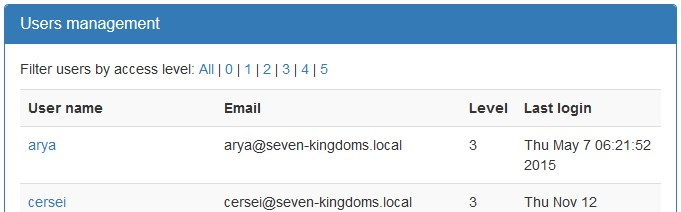
\includegraphics{userman.jpg}
\end{figure}

From there you can see a list of users, their email addresses, access levels, last logins along with the options to change their access levels and reset their passwords. Note that email notifications will only be sent out to users who confirmed their email addresses. This panel also allows passwords to be reset. You can see a summary page about a user by clicking on their names, and users can be disabled from that page.

Finally, new users can be created from that panel. If the \textbf{Allow Registrations} option is enabled, people can also register new user accounts from the login screen.

Here are the character restrictions for users:

\begin{itemize}
\item \textbf{User names:} Between 3 and 20 characters, using alphanumeric characters, plus the dot and dash. User names are not case sensitive during login authentication.
\item \textbf{Passwords:} At least 6 characters.
\item \textbf{Email addresses:} At the most 99 characters.
\end{itemize}

\subsection{Active Directory integration}
Active Directory integration can be enabled in the initial configuration, which will link the users management panel to your domain controller. Passwords will no longer be stored in the NodePoint database. Once a user attempts to login, their credentials will be validated, then NodePoint will check if a user entry exists in the database. A new entry will be created on first login. Users still need to set their email addresses for email notifications to work. Access levels can still be assigned to users to control their access to the NodePoint interface.

Authentication uses the LDAP protocol. You must specify a valid domain controller hostname or IP address for logins to work. If a login fails, you can view the log on the \textbf{System log} page to see the error message.

\subsection{Reports}
User activity can be monitored through two graphs along with a number of reports. The first graph shows the number of tickets entered per day for the last 7 days. The second one shows an overview of all tickets based on status. A calendar will also show time spent on tickets, due tasks and item expiration dates. Reports can be shown on the screen or downloaded as CSV documents to open in a spreadsheet application. Both are available to users of level 2 and higher (configurable) on the \textbf{Statistics} page.

\begin{figure}[h]
\includegraphics{reports.jpg}
\end{figure}

\clearpage
\section{Components}
NodePoint is divided into multiple components that you can enable or disable in the configuration as a product administrator. You can turn them on or off depending on your needs. For example, a help desk portal could have the \textbf{Tickets Management}, \textbf{Time Tracking} and \textbf{Support Articles} components enabled, while a project management portal could have only the \textbf{Tasks Management} component enabled.

\subsection{Tickets Management}
Users who have an access level of 1 or higher can enter tickets on the \textbf{Tickets} page. The default form asks for a title and description. Custom forms can also be designed and assigned to projects by users of access level 4 (configurable) and above. These custom forms can have up to 10 fields, each field can be a text area, a check box, satisfaction rating, priority, and so on. Projects that have a custom form assigned will display that form to users instead of the default one.

Users with access level 3 or above can modify tickets. When a ticket is modified, the description is updated to show who modified it, and what parameters were changed, such as the title, description, status and resolution. Open tickets do not require a resolution, but each other status does. The list of tickets can be filtered based on project, status and so on.

\subsubsection{Custom forms}
To use custom forms, follow these steps:

\begin{enumerate}
\item Add at least one project on the \textbf{Projects} page.
\item Create a custom form on the \textbf{Custom forms} page.
\item Assign that form to the project.
\end{enumerate}

Here is an example of a custom form being built along with the result:

\begin{figure}[h]
\includegraphics[scale=0.5]{customform.jpg}
\includegraphics[scale=0.5]{customform2.jpg}
\end{figure}

\subsubsection{Following and assignment}
Any logged in user can follow a ticket by clicking the proper option on the ticket's screen, which will add that ticket to their home screen for easy reference. This is meant as a way to follow an issue you are not actively working on.

Users with access level 3 or higher can assign themselves to a ticket by clicking the proper checkbox on the ticket's screen. This is meant as a way to assign resources to a particular issue.

Auto assignment can also be used to assign specific users to any ticket filed against a project. You can add yourself to the auto-assign list of a product by clicking the button on the project's screen:

\begin{figure}[h]
\includegraphics{autoassign.jpg}
\end{figure}

Both followed and assigned tickets are listed on the user's home page. Finally, email notifications are sent out when a ticket is created, modified or a comment is added. The notifications are sent to the ticket author and users assigned to that ticket.

\subsection{Support Articles}
The \textbf{Articles} page hosts articles that can be used to document common use cases, common issues, or to build a knowledge base for your organization. Articles are created in \textit{draft} mode, which hides them from users with an access level lower than 4. Only once they are published are they visible to all users.

Users with at least access level 3 can link articles to tickets. These can be used to assign related documentation to issues, or used as categories. Linked tickets (except closed ones) are listed on the article's page, which makes it easy to track which tickets are assigned to a specific article.

\subsection{Time Tracking}
When updating a ticket, users can track the time they spent on the issue, which will be added to the time table for that ticket. A total of all the time spent on tickets by a specific user is shown on the \textbf{Settings} page. A report is also available with the total time spent by all users.

Time entries cannot be removed since it acts as a timestamp for work done. Corrections can be made by entering negative values.

\subsection{Shoutbox}
The shoutbox is a simple chat area on the home page that all users can use. The box shows the last few entries made by users, and individual entries can be deleted by users with access level 5 or higher.

\subsection{Tasks Management}
The tasks management component can be used to manage products or projects, create new tasks needed to be completed, and assign these tasks to users with due dates. Users with access level 4 (configurable) or higher can create new tasks on the \textbf{Projects} page:

\begin{figure}[h]
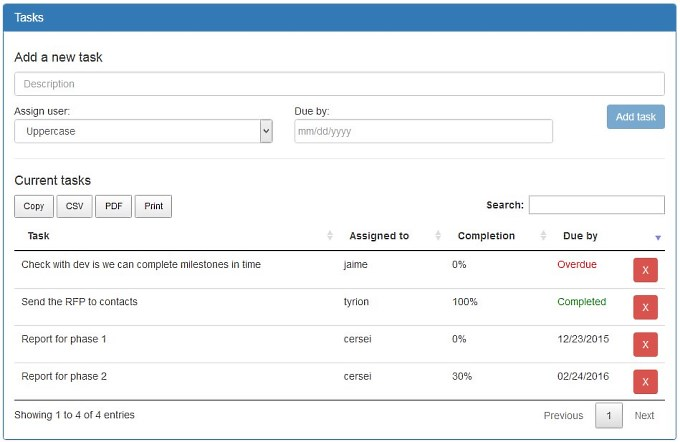
\includegraphics{projectmanagement.jpg}
\end{figure}

New tasks created will send an email notification to the user assigned to the task, and all tasks will show on the user's home page. There, users can modify the completion rate for each item. Completed and overdue tasks will also be highlighted.

\subsection{Clients Directory}
The clients directory can be used to keep track of clients or contacts from the \textbf{Clients} page. New clients can be added along with specific information such as email, phone number or notes by users of access level 5, details seen by users of level 2 (configurable) and higher. The following statuses can be assigned to clients:

\begin{itemize}
\item \textbf{Prospect:} A prospective client.
\item \textbf{Supplier:} A vendor.
\item \textbf{Contact:} A contact entry.
\item \textbf{Paid:} A paid client.
\item \textbf{Unpaid:} An unpaid or default client.
\item \textbf{Closed:} A closed entry (no ticket can be filed against closed clients).
\end{itemize}

If the clients directory is enabled, the \textit{Clients} field type can be added to custom ticket forms, which will show a drop down list of available clients when creating new tickets, to assign issues to specific clients. Events can be added by users of the right access level to log phone calls, emails and other communications. This can be used as a CRM portal to keep track of interactions with clients. 

\subsection{Inventory Control}
The Inventory Control component allows users with access level 4 or higher to add items to the \textbf{Items} page. These items can be linked to projects or clients, and can be checked out by other users. Approval can also be required, in which case users will need to request access, and someone with access level 4 or higher will need to approve the request. This component can be used to keep track of physical items such as computers, keyboards and phones, or even software licenses:

\begin{figure}[h]
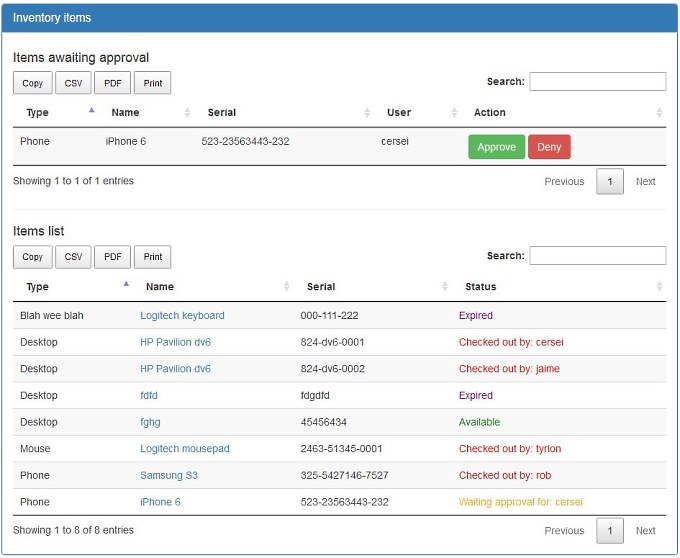
\includegraphics{items.jpg}
\end{figure}

When a user checks out an item, additional information such as item location, lock codes or other secret data can be displayed on the item's page and sent through email to that user, so that the person can retrieve it. This information field is otherwise hidden from other users. If approval is required, a notification will be sent to all available users with level 4 or higher. They can then decide to approve or deny the request. Items can have an expiration date, after which checkouts will be disabled.

Users with checked out items will see a list of items on their home page, and can then return the item, making it available to other users. A checkout history is kept for each item and shown on the item page, showing all past requests and events. Items can also be manually assigned to users, or made unavailable, preventing any user from requesting or checking them out.

An \textit{items} field is available to be used in custom ticket forms, which will display a list of checked out items that the user can file tickets about. Finally, a checkout plugin can be used to accomplish some automated task when an item is checked out, approved or assigned to a user.

\subsection{Files Management}
NodePoint provides a files upload feature for things like project images and file attachments to comments. If you enable the Files Management component, an option will be available under the \textbf{Tools} menu for users to upload arbitrary files as well. These files will be listed on that page, along with a direct link to download them, which can be used to send to clients or partners who may not have a user account configured:

\begin{figure}[h]
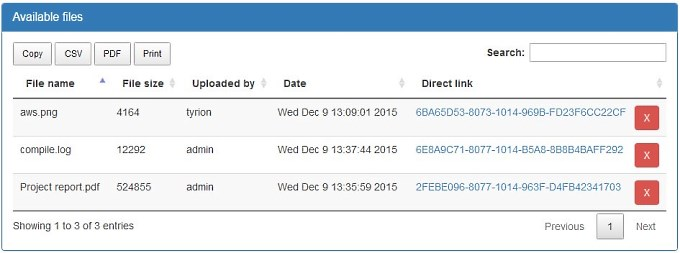
\includegraphics{files.jpg}
\end{figure}

Note that the files uploaded here, along with those attached to projects or tickets, must be below the configured maximum file size value. Also, only users with an access level above the one configured in the initial settings will be able to upload files. The files themselves will be available to anyone with the link.

\subsection{Billing}
The Billing component allows you to assign tickets to clients with either a fixed rate or an hourly rate. As such, this component requires the Tickets Management and Clients Directory components to be enabled. For hourly rates, the Time Tracking component must also be enabled.

When editing a ticket, a user of level 3 of higher can select a client from the drop down list, among clients that have been entered in the directory. Once tickets have been assigned to a client, the list of tickets with hours spent are listed on that client's page. The cost and currency can also be adjusted on that page.

\subsection{Automation}
NodePoint ships with an automation engine called \textbf{nodepoint-automate}. This engine is set as a scheduled task during the installation process, and controls the background automation modules, processes that can run without user intervention. Each module can be enabled or disabled individually, and scheduled on its own schedule of 5 minutes, 15 minutes, hourly, daily or weekly. Configuration is done under the \textbf{Tools} menu by users with the right access level.

These are the available automation modules:

\subsubsection{Backup}

This module allows you to backup the database along with the uploads folder to another location for safe keeping. The folder must be a local path, and the type of backup can be a single archive file or a series of time stamped files.

\subsubsection{Email to Ticket}

\subsubsection{Bulk import}

\subsubsection{Bulk export}

\subsubsection{Users sync}

\clearpage
\section{JSON API}
NodePoint provides a JSON based REST API that can be used to accomplish some basic tasks. This can be useful to integrate the system with existing products, or to use with custom scripts. Each API call requires either the \textit{read} or \textit{write} key. The calls can be made using GET or POST.

Here is a list of commands. Arguments in \textit{italics} are optional:

\subsection{List users}

\begin{itemize}
\item api=list\_users
\item key=<read key>
\end{itemize}

\subsection{Add new user}

\begin{itemize}
\item api=add\_user
\item key=<write key>
\item user=<user name>
\item password=<password>
\item email=<email>
\end{itemize}

\subsection{Verify user password}

\begin{itemize}
\item api=verify\_password
\item key=<read key>
\item user=<user name>
\item password=<password>
\end{itemize}

\subsection{Change user password}

\begin{itemize}
\item api=change\_password
\item key=<write key>
\item user=<user name>
\item password=<password>
\end{itemize}

\subsection{List tickets by product}

\begin{itemize}
\item api=list\_tickets
\item key=<read key>
\item product\_id=<product id>
\end{itemize}

\subsection{Show ticket}

\begin{itemize}
\item api=show\_ticket
\item key=<read key>
\item id=<ticket id>
\end{itemize}

\subsection{Add release}

\begin{itemize}
\item api=add\_release
\item key=<write key>
\item product\_id=<product id>
\item release\_id=<release id>
\item notes=<notes>
\end{itemize}

\subsection{Add ticket}

\begin{itemize}
\item api=add\_ticket
\item key=<write key>
\item product\_id=<product id>
\item release\_id=<release id>
\item title=<ticket title>
\item description=<ticket description>
\item \textit{priority=<Low|Normal|High>}
\item \textit{from\_user=<valid user>}
\end{itemize}

\subsection{Update ticket}

\begin{itemize}
\item api=update\_ticket
\item key=<write key>
\item id=<ticket id>
\item \textit{summary=<summary of changes>}
\item \textit{status=<New|Open|Invalid|Hold|Duplicate|Resolved|Closed>}
\item \textit{resolution=<new resolution>}
\item \textit{priority=<Low|Normal|High>}
\item \textit{time\_spent=<number of hours>}
\item \textit{from\_user=<valid user>}
\end{itemize}

\subsection{Add comment}

\begin{itemize}
\item api=add\_comment
\item key=<write key>
\item id=<ticket id>
\item comment=<comment>
\end{itemize}

\subsection{Show time tracking}

\begin{itemize}
\item api=show\_time
\item id=<ticket id>
\item key=<read key>
\end{itemize}

\subsection{Show billing information}

\begin{itemize}
\item api=show\_billing
\item client=<client name>
\item key=<read key>
\end{itemize}

\subsection{Add task}

\begin{itemize}
\item api=add\_task
\item key=<write key>
\item product\_id=<product id>
\item description=<task description>
\item user=<assigned user>
\item due=<mm/dd/yyyy>
\end{itemize}

\subsection{List tasks}

\begin{itemize}
\item api=list\_tasks
\item key=<read key>
\item user=<user>
\end{itemize}

\subsection{Add client}

\begin{itemize}
\item api=add\_client
\item key=<write key>
\item name=<client name>
\item status=<client status>
\item contact=<contact address>
\item \textit{notes=<notes>}
\end{itemize}

\subsection{List clients}

\begin{itemize}
\item api=list\_clients
\item key=<read key>
\end{itemize}

\subsection{List client events}

\begin{itemize}
\item api=list\_events
\item key=<read key>
\item client\_id=<client id>
\end{itemize}

\subsection{Add client event}

\begin{itemize}
\item api=add\_event
\item key=<write key>
\item client\_id=<client id>
\item summary=<event summary>
\item type=<event type>
\item \textit{notes=<notes>}
\item \textit{from\_user=<valid user>}
\end{itemize}

\subsection{Add item}

\begin{itemize}
\item api=add\_item
\item key=<write key>
\item product\_id=<0|product id>
\item client\_id=<0|client id>
\item approval=<0|1>
\item type=<item type>
\item name=<item name>
\item serial=<serial number>
\item info=<additional information>
\end{itemize}

\subsection{List items}

\begin{itemize}
\item api=list\_items
\item key=<read key>
\end{itemize}

\subsection{Assign item}

\begin{itemize}
\item api=assign\_item
\item key=<write key>
\item id=<item id>
\item user=<user>
\end{itemize}

\subsection{Return item}

\begin{itemize}
\item api=return\_item
\item key=<write key>
\item id=<item id>
\end{itemize}

\subsection{Update item}

\begin{itemize}
\item api=update\_item
\item key=<write key>
\item id=<item id>
\item \textit{product\_id=<product id>}
\item \textit{client\_id=<client id>}
\item \textit{approval=<0|1>}
\item \textit{type=<item type>}
\item \textit{name=<item name>}
\item \textit{serial=<serial number>}
\item \textit{info=<additional information>}
\item \textit{expiration=<mm/dd/yyyy>}
\end{itemize}

\subsection{Code example}
The following code snippet is a Python 3.x example of how to access the API. This script connects to a local NodePoint instance and lists all the users:

\begin{lstlisting}
import json
import urllib.request
import urllib.parse

post_params = {'api': 'list_users', 'key': '0qvG4DkOz8NZnkuhn4aczck7r3qQVYS4'}

post_args = urllib.parse.urlencode(post_params)
data = post_args.encode()
stream = urllib.request.urlopen('http://localhost/nodepoint/', data)
result = stream.read()
charset = stream.info().get_param('charset', 'utf8')
users = json.loads(result.decode(charset))
for user in users['users']:
    print(user['name'])
\end{lstlisting}

\clearpage
\section{License}
The MIT License (MIT)

Copyright \textcopyright \thinspace 2014-\the\year \thinspace Patrick Lambert

Permission is hereby granted, free of charge, to any person obtaining a copy
of this software and associated documentation files (the "Software"), to deal
in the Software without restriction, including without limitation the rights
to use, copy, modify, merge, publish, distribute, sublicense, and/or sell
copies of the Software, and to permit persons to whom the Software is
furnished to do so, subject to the following conditions:

The above copyright notice and this permission notice shall be included in
all copies or substantial portions of the Software.

THE SOFTWARE IS PROVIDED "AS IS", WITHOUT WARRANTY OF ANY KIND, EXPRESS OR
IMPLIED, INCLUDING BUT NOT LIMITED TO THE WARRANTIES OF MERCHANTABILITY,
FITNESS FOR A PARTICULAR PURPOSE AND NONINFRINGEMENT. IN NO EVENT SHALL THE
AUTHORS OR COPYRIGHT HOLDERS BE LIABLE FOR ANY CLAIM, DAMAGES OR OTHER
LIABILITY, WHETHER IN AN ACTION OF CONTRACT, TORT OR OTHERWISE, ARISING FROM,
OUT OF OR IN CONNECTION WITH THE SOFTWARE OR THE USE OR OTHER DEALINGS IN
THE SOFTWARE.

\end{document}

